
%\vspace*{-0.4cm}
\section{Data Analysis using Jupyter}


\begin{figure*}[hbt!]
\centering
	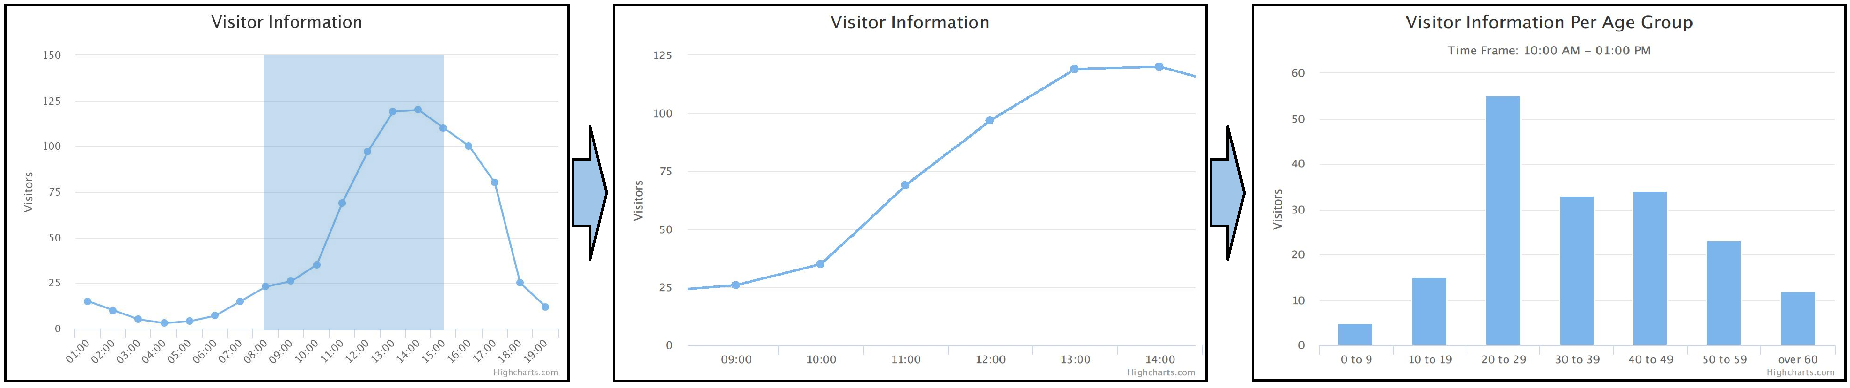
\includegraphics[width=1\textwidth]{figures/reactive-processing2.pdf}
	\caption{Demonstration of reactive charts. The reader's selection automatically updates both charts.}
	\label{fig:reactive-data-processing}
	\vspace{-6pt}
\end{figure*}



\costas{reviewer 1: c. Logging into databases, etc using Python libraries is not really harder today than what you show in the paper. See the ipython-sql library and its use of SQLAlchemy. For us database folks, this is already a standard way to work with Python and notebooks. d. You seem to indicate that there is an unsolved object-relational data type conversion problem in Python/SQL. But Pandas dataframes do a fine job with this, even over something like ipython-sql. This is a non-issue for Python notebook users today. }

\costas{ipython-sql is a python magic command that let's you inline queries in Jupyter and it returns the result in a pandas dataframe. This tool lacks the interactive aspect which is required in order to build a reactive analysis. You cannot issue a parameterized query that is executed every time the user interacts with a visualization (I verified this).}


We will now describe how a data scientist would perform this analysis with a traditional interactive notebook and illustrate how the limited interactive capabilities affect the level of data exploration that can be performed. We assume that the news portal maintains data about its reader-base in a Postgres database. Table \ref{tab:schema} shows a potential schema, that could be used for storing visitor information. The database contains two tables, namely ``Page Views" and ``Visitors"; table ``Visitors" contains information about each reader, such as the reader id, name, lastname, username, age and gender. The table ``Page Views" maintains a tuple for each visit, and it consists of a visit id, the visitor id (foreign key referencing the visitor), the url of the visited page, the hour and date in which the user visited the website and the revenue collected during this visit. The reader information could have been retrieved, with their permission, from various social media services (such as Facebook, Google etc). 

\noindent {\bf Data analysis steps.}
In order to construct this notebook, the data analyst must (a) retrieve  website access information from the database, by joining the two tables on the visitor id (b) generate a plot that shows the number of users that visit the website during the day, (c) issue a query that counts the number of visitors per age group for a meaningful set of hours (time frame), (d) create a bar chart that shows the number of visitors per age group, (e) use an already trained predictive model in order to predict the expected revenue for the selected time window and (f) plot a bar chart, showing the actual and the predicted revenue generated in selected time window. Note that in order to perform these steps, the data analyst must employ a plethora of third-party Python libraries (database drivers, machine learning and visualization libraries etc.,) used for data access, data processing and visualization. Each of those libraries expects or returns data in a predefined schema, therefore, the analyst must manually perform schema transformations for each library they want to use. Most importantly, note that selecting a meaningful time frame (step c) in this analysis, is of utmost significance, because it will affect all the remaining steps of this analysis, and ultimately the insight, the portal editor will gain, about potential ways to increase the revenue

 \eat{
In order to retrieve website access information from the database, the data analyst, needs to employ third-party Python drivers. After establishing the connection with the database system, and issuing the queries, the analyst, is able to consume the results using the internal, to the library, data types. Afterwards, the analyst needs to perform (schema) conversions in order to invoke the respective visualization library, with the appropriate arguments, thus constructing the first visualization.
}

\costas{Repeating comment here: d. You seem to indicate that there is an unsolved object-relational data type conversion problem in Python/SQL. But Pandas dataframes do a fine job with this, even over something like ipython-sql. This is a non-issue for Python notebook users today. Separate comment: It felt to me that you are unfamiliar with Jupyter Lab, Pandas, and the rest of the standard toolchain that people use. Maybe that's not true! But it comes across that way. For example, it's odd that you return dictionaries rather than dataframes, and your comments on "Data conversion" reinforces that feeling. If you do know your stuff, then for some reason you are not integrating with the community's favorite libraries. If that's the case, you might be more thoughtful in explaining why your counter-cultural approach is good.}

\costas{The point I was trying to make here is that regardless of whether we integrate with dictionaries or dataframes, the analyst still has to read the documentation page of the visualization library and manually convert the data into the format/schema that is expected by the visualization library. Dataframes are indeed used a lot by many libraries however they cannot capture nested data while dictionaries can. Additionally, dictionaries are natively supported by Python while Pandas is an external library. Also while some tools interface well with pandas many of them actually require conversions into python dictionaries/arrays (here is an example using plotly that requires a dataframe to be converted into a dictionary: https://plot.ly/ipython-notebooks/cufflinks/, plotly has the same issue) as shown in the same link because of this missmatch, additional libraries have to be used to simplify this data conversion (i.e., cufflinks). On the other hand all libraries interface with python natively supported types (i.e., dictionaries) additionally dataframes can be converted into (flat) dictionaries with one command (and the other way around)... If he considers integration with dataframes (which again are simply flat dictionaries) so critical, we can support that as well. On a separate note, Jupyter Labs is simply a more advanced web IDE for creating ipython notebooks. I don't understand how that's comparable to vidette (one can use Jupyter labs to build a jupyter notebook that employs vidette...)}

\eat{
The next step is for the analyst to issue a query that counts the visitors per age group for a set of selected hours and construct a bar chart showing the result. The obtained dataset will also go through a machine learning package (for instance, the scikit-learn package \cite{scikit-learn}), that employs a linear regression model to predict the expected revenue during the selected hours. The predicted revenue will be plotted in a new graph next to the actual revenue produced during these hours. Note that selecting a meaningful time frame, is of utmost importance, because it will affect all the remaining steps of this analysis, and ultimately the insight, the portal editor will gain, about potential ways to increase the revenue. 
}




 % Template and template instance figures
 \begin{figure*}[hbt!]
 \centering
 %
 %
 \begin{minipage}[c]{7cm}
 %
 \begin{minipage}[c]{7cm}
 \begin{code}
 \textbf{<\% let} readings = sql(
    SELECT count(time) as visits, time
    FROM (SELECT * FROM page_views pv 
   	     join visitors v 
          on pv.v_id = v.vid) AS joined_table
    GROUP BY time ORDER BY time ASC \textbf{\%>};)
 \end{code}
 \vspace*{-0.2cm}
 \subcaption{Data retrieval}
 \label{figure:first-running-example:data-retrieval}
 \vspace*{0cm}
 \end{minipage}
 
 
 \begin{minipage}[c]{7cm}
 	\begin{code}
 \directive{unit}{highcharts} \{
   title: 'Visitor information' , type: 'line',
   xAxis : \{ 
     labels : ['08:00','09:00'...], min : '08:00', max : '22:00'
   \}
   series: [\{ data: [ \{y:15\}, \{y:10\}...] \}]
 \} \directive{end unit}{}
 	\end{code}
 	\vspace*{-0.2cm}
 	\subcaption{Unit with evaluated unit state}
 	\vspace*{0cm}
 	\label{figure:running-example:unit-body}
 \end{minipage}
 \begin{minipage}[c]{7cm}
 	\begin{code}
 readings = [ \{visits: 15, time: '08:00'\},...]
 	\end{code}
 	\vspace*{-0.2cm}
 	\subcaption{Query Result}
 	\label{figure:running-example:query-result}
 	\vspace*{0cm}
 \end{minipage}
 %
 \vspace*{0cm}
 \end{minipage}
 \hspace{2cm}
 \begin{minipage}[c]{6cm}
 
 \begin{minipage}[c]{7.5cm}
 \begin{code}
   \directive{init}{min_time = '01:00'} 
   \directive{init}{max_time = '24:00"} 
   \directive{unit}{highcharts} \{
     title: 'Visitor information',
     type: 'line',
     xAxis : \{ 
       labels : [
         \directive{for}{reading \textbf{in} readings} 
           \directive{print}{reading.time} 
         \directive{end for}{}],
       min : \directive{bind}{min_time},
       max : \directive{bind}{max_time}
     \}
     series: [\{
       data: [ \directive{for}{reading \textbf{in} readings}
           \{
             y  : \directive{print}{reading.count}
           \}  
           \directive{end for}{} ]
     \}] \} \directive{end unit}{}
 \end{code}
 \vspace*{-0.2cm}
 \subcaption{Template generating unit state of first chart}
 \vspace*{0cm}
 \label{figure:first-running-example:main-template}
 \end{minipage}
 \end{minipage}
 \vspace*{-0.3cm}
 \caption{Declarative data retrieval, evaluated unit state and Template describing unit state for running example}
 \vspace*{-0.3cm}
 \end{figure*}
 
 \noindent {\bf Limited interactivity impacts exploratory capabilities.} Unfortunately, there is no straightforward way for selecting a meaningful time frame. The analyst will have to go through a process of trial and error, by issuing an arbitrary number of such queries and plotting the results, until she finds a set that produces valuable insight. Furthermore, even if the analyst goes through this process for the data corresponding to a particular day, the time frame selection they made, might not produce any valuable insight for the dataset corresponding to a different day. Most importantly the non-technical readers cannot use the notebook to test similar hypotheses, they are limited to passively reading the ones that were hardcoded by the analyst. This aspect of introducing the human in the loop is improved dramatically with \projname\ notebooks.
 

